% -----------------------------------------------
% Template for JIM
%     jim.sty -> style file
% By Eloi Batlle (eloi@iua.upf.es), changes for 
% ICMC by Bram de Jong (bdejong@iua.upf.es)
% changes for JIM 2007 by Dominique Fober (fober@grame.fr)
% changes for JIM 2009 by Olivier Tache (olivier.tache@imag.fr)
% -----------------------------------------------

\documentclass{article}
\usepackage{jim,amsmath}
\usepackage[utf8]{inputenc}
\usepackage[francais]{babel}
\usepackage[T1]{fontenc}
%\usepackage{pxfonts}
\usepackage{graphicx}
\usepackage{balance}

\usepackage{verbatim}
\usepackage{color}
\usepackage{textcomp}

% Title.
% ------
\title{Composition de partitions symboliques dnas INScore}

% Single \textsc{address}
% To use with only one author or several with the same address
% ---------------
%\oneauthor
%  {Author} {School \\ Department}

% Two addresses
% --------------
%\twoauthors
%  {First author} {School \\ Department}
%  {Second author} {Company \\ Address}

% Three addresses
% --------------
\threeauthors
  {Auteur 1} {Organisme \\ Adresse électronique}
  {Auteur 2} {Organisme \\ Adresse électronique}
  {Auteur 3} {Organisme \\ Adresse électronique}

\begin{document}
%
\maketitle
%
\begin{abstract}
Le résumé doit être placé en haut de la colonne gauche et doit contenir entre 150 et 200 mots.
\end{abstract}
%
\section{Introduction}\label{sec:introduction}

Ce modèle précise les règles pour une bonne présentation des communications à proposer aux JIM 2012. Il s'inspire du modèle proposé par l'ICMC 2005.

Merci de le suivre afin de permettre une présentation unifiée des actes. 


\section{Taille de la page}\label{sec:page_size}

Les actes seront imprimés au format A4 (21 x 29.7 cm). Le contenu de chaque page doit pouvoir tenir dans un rectangle de (17 x 24.7 cm) centré sur la page, commençant à 2 cm du haut de la page et s'arrêtant à  3 cm du bas de la page. Les marges gauche et droite doivent être de 2 cm. Le texte est présenté sur deux colonnes (8,1cm) avec une gouttière  de 0,8 cm. Le texte doit être justifié à gauche et à droite.

\section{Police de caracteres}\label{sec:typeset_text}

\subsection{Corps du texte}\label{subsec:body}

Utiliser la police Times 10 pt (points). N'utiliser une police sans serif ou non proportionnelle que pour des raisons particulières, par exemple pour distinguer des lignes de code du reste du texte.

\subsection{Titre et auteurs}

Le titre est en Times 14 pt, gras, majuscule, centré. Les noms des auteurs sont centrés. Si l'adresse est la même pour tous les auteurs, elle ne doit figurer qu'une seule fois, centrée. Dans le cas contraire, elle doit apparaître sous le nom de chaque auteur.

\subsection{Numéro de page, haut de page et  bas de page}

Ne pas inclure  de numéro de page, de haut de page ou de bas de page lors de votre soumission. Ils seront ajoutés par l'éditeur.

\section{Sections}

Les titres de sections sont en Times, 10 pt gras, centrés avec 1 ligne d'espace au-dessus du titre de section, et 1/2 espace au-dessous. Pour un titre de section immédiatement suivi d'un titre de sous-section, ne pas additionner les deux espaces.

\subsection{Sous-sections}

Les titres de sous-sections sont en Times 10 pt alignés à gauche, avec une ligne d'espace au-dessus, et 1/2 ligne d'espace au-dessous.

\subsubsection{Sous-sous-sections}

Les sous-sous-sections sont en Times 10 pt italique, alignés à gauche, avec 1 ligne d'espace au-dessus et 1/2 ligne d'espace au-dessous.

On évitera d'utiliser plus de trois niveaux de section.


\section{Notes de bas de page et Figures}

\subsection{Notes de bas de page}

Indiquer la note de bas de page avec un numéro dans le texte\footnote{Ceci est une note de bas de page}.  Utiliser la police Times 8 pt. Placer les notes en bas de chaque page où elles vont apparaitre. Faire précéder la note d'une ligne horizontale de 0,5 pt.

\subsection{Illustrations, figures et tableaux}

Toutes les illustrations devront être centrées dans une colonne, propres et lisibles (Figure 1). L'impression des actes sera en noir et blanc. Les figures doivent donc faire sens en noir et blanc. Les numéros de figure, de tableau et leur légende doivent toujours apparaître en dessous de la figure. Laisser une ligne d'espace entre la figure et sa légende. Chaque figure ou tableau est numéroté consécutivement. Les légendes seront présentées en Times 10 pt et indentées. Placer les illustrations aussi près des références que possible. Elles peuvent être placées au centre de la page, traversant les deux colonnes, dans une limite de 17cm.

\begin{table}
\begin{center}
\begin{tabular}{|l|l|}
\hline
Texte & Valeur \\
\hline
hello jim  & 1073 \\
\hline
\end{tabular}
\end{center}
\caption{La légende du tableau devra être placée sous le tableau.}
\label{tab:example}
\end{table}

%\begin{figure}
%\centerline{\framebox{
%	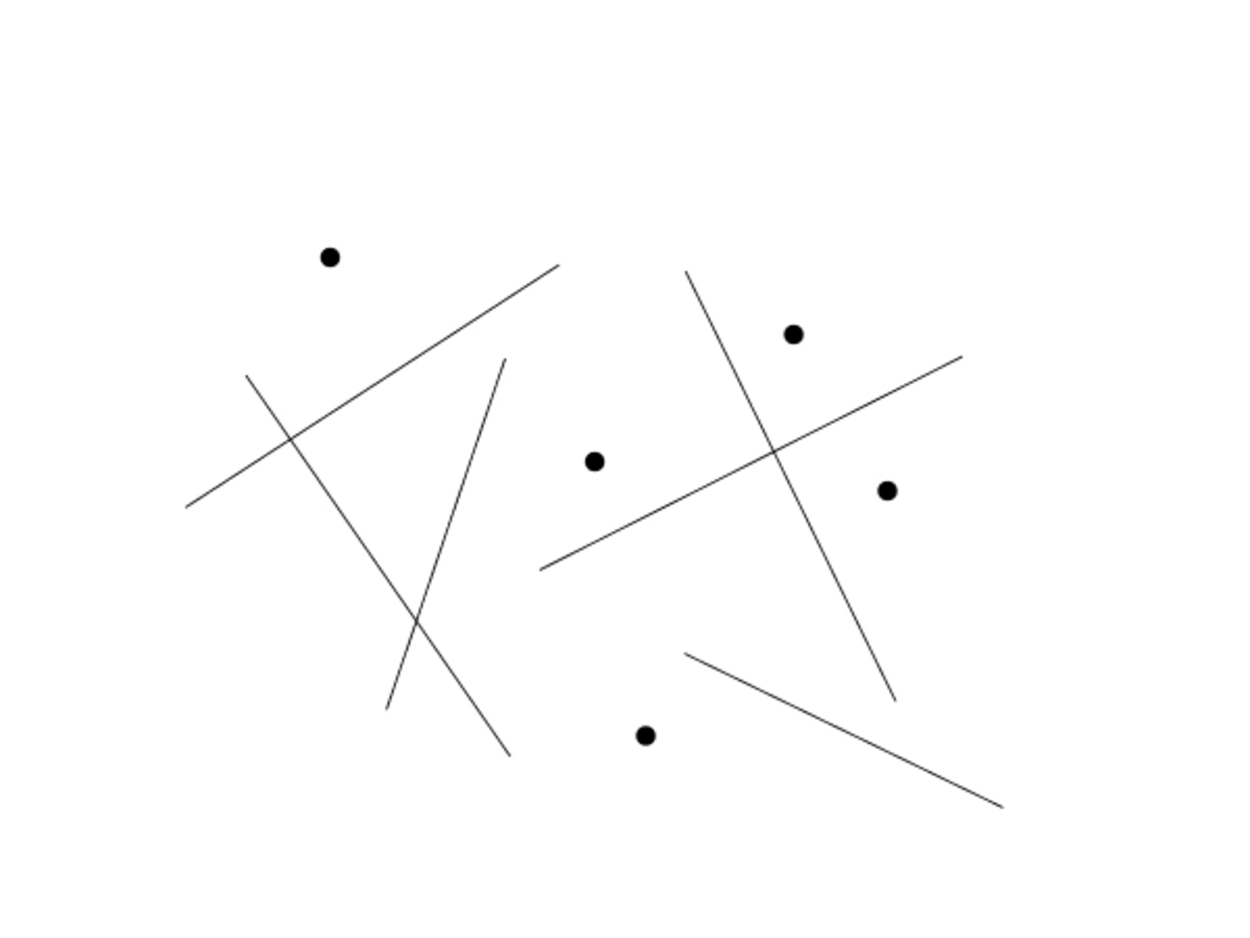
\includegraphics[width=\columnwidth]{figure}}}
%\caption{La légende de la figure devra être placée sous la figure.}
%\label{fig:example}
%\end{figure}

\section{Equations}

Les équations devront être placées sur des lignes séparées et numérotées. Le numéro devra être placé à droite.

\begin{equation}
E=mc^{2}
\end{equation}

\section{Citations}

Toutes les références bibliographiques des citations devront être listées dans la section "\textsc{References}", numérotées et en ordre alphabétique. Toutes les références  listées devront être citées dans le texte. Quand  vous vous référez au document dans le texte, précisez son numéro \cite{Author:00}.

%\balance
\bibliography{../interlude}

\end{document}
